% $Id: template.tex 11 2007-04-03 22:25:53Z jpeltier $

%\documentclass{vgtc}                          % final (conference style)
\documentclass[review]{vgtc}                 % review
%\documentclass[widereview]{vgtc}             % wide-spaced review
%\documentclass[preprint]{vgtc}               % preprint
%\documentclass[electronic]{vgtc}             % electronic version

%% Uncomment one of the lines above depending on where your paper is
%% in the conference process. ``review'' and ``widereview'' are for review
%% submission, ``preprint'' is for pre-publication, and the final version
%% doesn't use a specific qualifier. Further, ``electronic'' includes
%% hyperreferences for more convenient online viewing.

%% Please use one of the ``review'' options in combination with the
%% assigned online id (see below) ONLY if your paper uses a double blind
%% review process. Some conferences, like IEEE Vis and InfoVis, have NOT
%% in the past.

%% Figures should be in CMYK or Grey scale format, otherwise, colour 
%% shifting may occur during the printing process.

%% These three lines bring in essential packages: ``mathptmx'' for Type 1 
%% typefaces, ``graphicx'' for inclusion of EPS figures. and ``times''
%% for proper handling of the times font family.

\usepackage{mathptmx,ifpdf}
\usepackage{graphicx}
\usepackage{times}

%% We encourage the use of mathptmx for consistent usage of times font
%% throughout the proceedings. However, if you encounter conflicts
%% with other math-related packages, you may want to disable it.

%% If you are submitting a paper to a conference for review with a double
%% blind reviewing process, please replace the value ``0'' below with your
%% OnlineID. Otherwise, you may safely leave it at ``0''.
\onlineid{0}

%% declare the category of your paper, only shown in review mode
\vgtccategory{Research}

%% allow for this line if you want the electronic option to work properly
\vgtcinsertpkg

%% In preprint mode you may define your own headline.
%\preprinttext{To appear in an IEEE VGTC sponsored conference.}

%% Paper title.

\title{Identifying Inexpensive Off-the-Shelf Laser Pointers for \\ Multi-User Interaction on Large Scale Displays}

%% This is how authors are specified in the conference style

%% Author and Affiliation (single author).
%%\author{Roy G. Biv\thanks{e-mail: roy.g.biv@aol.com}}
%%\affiliation{\scriptsize Allied Widgets Research}

%% Author and Affiliation (multiple authors with single affiliations).
%%\author{Roy G. Biv\thanks{e-mail: roy.g.biv@aol.com} %
%%\and Ed Grimley\thanks{e-mail:ed.grimley@aol.com} %
%%\and Martha Stewart\thanks{e-mail:martha.stewart@marthastewart.com}}
%%\affiliation{\scriptsize Martha Stewart Enterprises \\ Microsoft Research}

%% Author and Affiliation (multiple authors with multiple affiliations)
\author{Christopher Stuetzle\thanks{e-mail: christopher.stuetzle@gmail.com}\\ Rensselaer Polytechnic Institute \\ Computer Science Dept. %
\and Barbara Cutler\thanks{e-mail: cutler@cs.rpi.edu}\\ Rensselaer Polytechnic Institute \\ Computer Science Dept. %
%\and Andrew Dolce\thanks{e-mail:andrew@gradient-studios.com}\\ Gradient Studios %
%\and Patrick Phipps\thanks{e-mail:phippp@rpi.edu}\\ RPI Computer Science Dept. %
%\and Joshua Nasman\thanks{e-mail:nasmaj@cs.rpi.edu}\\ RPI Computer Science Dept. %
%\and Andrew Zonenberg\thanks{e-mail:zonena@rpi.edu}\\ RPI Computer Science Dept.
%\and W. R. Franklin\thanks{e-mail:franklin@cs.rpi.edu}\\ RPI ECSE Dept. %
%\and Ryan Baltazar\thanks{e-mail:baltar@rpi.edu}\\ RPI Computer Science Dept. % 
}


% \author{Roy G. Biv\thanks{e-mail: roy.g.biv@aol.com}\\ %
%        \scriptsize Starbucks Research %
% \and Ed Grimley\thanks{e-mail:ed.grimley@aol.com}\\ %
%     \scriptsize Grimley Widgets, Inc. %
% \and Martha Stewart\thanks{e-mail:martha.stewart@marthastewart.com}\\ %
%     \parbox{1.4in}{\scriptsize \centering Martha Stewart Enterprises \\ Microsoft Research}}


% WE SHOULD INCLUDE A TEASER IMAGE!
% A teaser figure can be included as follows, but is not recommended since
% the space is now taken up by a full width abstract.
% \teaser{
%  \includegraphics[width=1.5in]{images/paint.jpg}
%  \caption{\label{figure:paint}A visualization of the multi-user paint program demonstrating two-user collaboration. Notice that laser \#1 has currently been assigned the color white and is filling in the cloud, while laser \#2 has recently selected the ``undo'' function which removed its color assignment.}
% }

%% Abstract section.
\abstract{
%
We present a method for identifying inexpensive, off-the-shelf laser
pointers in a multi-user interaction environment on large-scale
displays. We identify a laser pointer's \textit{personality}, a
measure of its output in a particular context. Our method requires a
set of inexpensive and unmodified green lasers, a large screen, a
projector, and a camera with an infrared (IR) filter. The camera
detects the IR spillover from the green laser beam, while ignoring
color information projected onto the screen. During a calibration
phase, a radial histogram of each laser's IR 
%radius and brightness
spillover (datapoints taken over
several frames) are used to represent the 
%fit to a Gaussian and are used to determine the
laser's \textit{personality}. Using this signature, our system is able
to identify the spots of a specific laser, allowing multiple users to
simultaneously interact in the environment. In addition, we present a
series of applications that take advantage of tracked and identified
laser pointers to demonstrate the usefulness of large-scale,
multi-user interactions and the feasibility of providing such a system
inexpensively and without the hassle of additional laser pointer
modifications.
%
}
% end of abstract

%% ACM Computing Classification System (CCS). 
%% See <http://www.acm.org/class/1998/> for details.
%% The ``\CCScat'' command takes four arguments.

\CCScatlist{ 
  \CCScat{H.5.3}{Information Interfaces and Presentation}%
{Group and Organization Interfaces}{Collaborative Computing};
%   \CCScat{K.7.m}{The Computing Profession}{Miscellaneous}{Ethics}
}

%% Copyright space is enabled by default as required by guidelines.
%% It is disabled by the 'review' option or via the following command:
% \nocopyrightspace

%%%%%%%%%%%%%%%%%%%%%%%%%%%%%%%%%%%%%%%%%%%%%%%%%%%%%%%%%%%%%%%%
%%%%%%%%%%%%%%%%%%%%%% START OF THE PAPER %%%%%%%%%%%%%%%%%%%%%%
%%%%%%%%%%%%%%%%%%%%%%%%%%%%%%%%%%%%%%%%%%%%%%%%%%%%%%%%%%%%%%%%%

\begin{document}

%% The ``\maketitle'' command must be the first command after the
%% ``\begin{document}'' command. It prepares and prints the title block.

%% the only exception to this rule is the \firstsection command
\firstsection{Introduction}

\maketitle

Multi-user, large-scale interfaces, in which individual users are
identified and tracked, present a challenging and worthwhile design
problem. In applications in which efficient interactivity between
users is important, laser pointer devices are preferable to stationary
pointer devices, such as
mice~\cite{Pavlovych:2008:ESC:1462027.1462035}. In most cases, the
challenge of identifying individual users is tackled by physically
modifying laser pointers, an effective yet often-times costly and
time-consuming solution.  To circumvent these drawbacks, we present
the idea of describing a laser by its \emph{personality}, a measure of
the shape and intensity of a laser pointer's leaked infrared light,
which allows us to track and identify an off-the-shelf laser pointer
among a group of others for the purpose of multi-user collaborative
applications.
%Our system does not require that the laser pointers receive any modifications whatsoever, and so can be used off-the-shelf with the system.
%
%In addition, 
We also present a series of applications that take advantage of the laser
personality system to exhibit group problem solving, data
manipulation, and data exploration. 

Our contributions are: \vspace{-0.1in}

\begin{itemize}

\item The \emph{laser pointer personality}, the signature shape and
  intensity of a laser point's infrared light leak.\vspace{-0.1in}

\item The laser pointer personality system used to identify an
  off-the-shelf laser pointer\vspace{-0.1in}

\item Several multi-user applications that demonstrate the utility of
  the personality system
\end{itemize}

\subsection{Related Work}

Single laser point detection is accomplished in two main ways:
brightness filtering and infrared filtering. Olsen and Nelson detect a
laser spot on a large display screen with a two pass
system~\cite{olsen2001}. The first pass detects the brightest red spot
in the image, while the second (which only occurs if no obvious laser
spot is found) passes over the screen again, employing a convolution
filter, concentrating on the area where the last spot was detected. Oh
and Stuerzlinger allow for multiple laser points by applying a
threshold to the brightness field of the
image~\cite{Oh02laserpointers}. The same technique is applied by Davis
and Chen in their LumiPoint
system~\cite{Davis00lumipoint:multi-user}. However, depending on the
brightness of the laser spot with respect to the rest of the image can
create trouble, as it is context sensitive and simple thresholds may
confuse the laser points and very bright sections of the
image. Ahlborn, et al.~\cite{Ahlborn:2005:PSL:1101616.1101637} present
a system using multiple camera views, in which the background image is
filtered out, leaving only laser points for detection. IR filtering is
employed by work by Qin, et al.~\cite{Qin:2010:SLP:1842993.1843022},
Angelini, et al.~\cite{angelini:multi-user}, and Cheng, et
al.~\cite{Cheng:2003:DIL:857080.857088}.

\begin{figure}

\includegraphics[width=0.16\linewidth]{images/SpotPPMs/tagged_0_frame_492_point_FC_0.png}
\includegraphics[width=0.16\linewidth]{images/SpotPPMs/tagged_3_frame_728_point_FC_0.png}
\includegraphics[width=0.16\linewidth]{images/SpotPPMs/tagged_6_frame_977_point_FC_0.png}
\includegraphics[width=0.16\linewidth]{images/SpotPPMs/tagged_9_frame_1217_point_FC_0.png}
\includegraphics[width=0.16\linewidth]{images/SpotPPMs/tagged_12_frame_1484_point_FC_0.png}
\includegraphics[width=0.16\linewidth]{images/SpotPPMs/tagged_15_frame_1731_point_FC_0.png}%
\vspace{0.01in}

\includegraphics[width=0.16\linewidth]{images/SpotPPMs/tagged_1_frame_553_point_FC_0.png}
\includegraphics[width=0.16\linewidth]{images/SpotPPMs/tagged_4_frame_784_point_FC_0.png}
\includegraphics[width=0.16\linewidth]{images/SpotPPMs/tagged_7_frame_1038_point_FC_0.png}
\includegraphics[width=0.16\linewidth]{images/SpotPPMs/tagged_10_frame_1273_point_FC_0.png}
\includegraphics[width=0.16\linewidth]{images/SpotPPMs/tagged_13_frame_1536_point_FC_0.png}
\includegraphics[width=0.16\linewidth]{images/SpotPPMs/tagged_16_frame_1773_point_FC_0.png}%
\vspace{0.01in}

\includegraphics[width=0.16\linewidth]{images/SpotPPMs/tagged_2_frame_599_point_FC_0.png}
\includegraphics[width=0.16\linewidth]{images/SpotPPMs/tagged_5_frame_838_point_FC_0.png}
\includegraphics[width=0.16\linewidth]{images/SpotPPMs/tagged_8_frame_1085_point_FC_0.png}
\includegraphics[width=0.16\linewidth]{images/SpotPPMs/tagged_11_frame_1328_point_FC_0.png}
\includegraphics[width=0.16\linewidth]{images/SpotPPMs/tagged_14_frame_1594_point_FC_0.png}
\includegraphics[width=0.16\linewidth]{images/SpotPPMs/tagged_17_frame_1819_point_FC_0.png}

\vspace{-0.1in}
  \caption{\label{figure:laser_dots} 
False color renderings of the IR spill from 6 inexpensive green laser
pointers.  The pattern of this spill is relatively constant, allowing
us to track and identify the lasers over time.  The pattern of spill
from the laser varies most with distance of the laser to the screen.
The top row of images were collected with the laser ~15 feet from the
screen, the middle row was ~10 feet from the screen, and the bottom
row.  The second row was ~5 feet from the screen.
}
\end{figure}

In addition to laser spotting, one challenge in multi-user laser
pointer systems is pointer identification. One method is to
dynamically change the number of lasers present in the system at any
given point in time, and to track an IDed laser spot across frames
with predictive measures, such as the Kalman
filter~\cite{Oh02laserpointers,Davis00lumipoint:multi-user,Cheng:2003:DIL:857080.857088}.
Another method involves the use of time division multiplexing, or the
application of a laser blinking pattern, to identify a particular
laser. Given \emph{n} lasers, a system can force exactly one of the
lasers off each frame. With cameras with high frame rates, this
produces an unnoticeable effect with regard to the temporal coherence
of the laser spot on the screen, but the system can identify the laser
by its blinking pattern. This method is employed by Vogt, et
al.~\cite{Vogt:2004:ECG:1009379.1009663,Vogt03trackingmultiple}, as
well as Pavlovych and Stuerzlinger~\cite{Pavlovych04laserpointers}.

Laser point detection, both single- and multi-user, has a variety of
applications, most of which revolve around user collaboration and
interaction. Francisco de la O Chavez, et al., present a system
whereby users can operate the electronic devices and appliances in
their homes with a laser pointer~\cite{delaOChavez:2008:INL:1387269.1387276}. The system uses a
single camera, and the user sets up ``active zones'', or groups of
pixels in the camera view around each appliance. When a laser spot is
detected in the active zone, the appliance is activated. Qin, et al.,
present a system in which a special laser pointer is used to project
several beams, and the orientation of the beams indicates the angle of
rotation along the beam axis of the laser, thus allowing for gestures
and object manipulation that involves rotation~\cite{Qin:2010:SLP:1842993.1843022}. Bi, et al. present the uPen, a
laser pointer outfitted with right- and left-click buttons, designed
to mimic computer mouse functionality~\cite{BiUpen}.
Shizuki, et al.~\cite{Shizuki:2006:LPI:1133265.1133284} present a series of 
gestures used with a laser pointer, and a series of applications using them.
The gestures are edge-crossing gestures, and the applications presented include 
a presentation application using gestures to move slides forward, and a picture 
viewing application where gestures manipulate the images.

To our knowledge, no work has been published regarding the
identification of off-the-shelf laser pointers in multi-user
applications. Also, the domain of applications that have been explored
for multi-user laser pointer interaction is rather small, either due
to lack of need or due to the necessity of engineering laser pointers
to make the interfaces effective.


\section{Laser Pointer Personalities}
\label{section:LaserPersonalities}



\subsection{System Details}
\label{section:systemdetails}

To detect the current position of each laser pointer dot, we use a
1280 x 960 pixel monochrome, 33fps video camera.  An infrared (IR)
pass filter in front of the camera blocks all visible light (from the
projector), so we can robustly detect the bright points of IR light
from the laser.  We specifically use green laser pointers because the
green light is produced indirectly from an infrared laser diode, and
some of the infrared light remains for our detection.  Most
inexpensive green lasers do not include an IR filter to block this
light.

We begin with a simple
calibration step to determine the pixel to
pixel correspondence between our camera and the 1920 x 1080 projector
and 
%18' tall screen.  
projection surface, and to collect intensity data on all lasers in the system. Our system has been tested on screens as tall as 18'.
We simply shine a laser at a 3x4 grid of
calibration points.  The first geometric calibration
% DOES IT? I AM CONFUSED
allows us to identify
multiple lasers simultaneously pointed at the screen.  For non-erratic
laser motions, we can easily track these points over time to allow
users to perform actions within an application, for example {\em
  moving} pieces around in a jigsaw puzzle (Figure~\ref{figure:puzzle}) or
{\em circling} nodes in a graph visualization (Figure~\ref{figure:graphVisualization}).

When tracking multiple lasers simultaneously, we use the Kuhn-Munkres,
a.k.a. {\em Hungarian
  Algorithm}~\cite{kuhn,munkres,munkres_implementation} to match the
lasers from frame to frame.  This method produces a pairing that
efficiently minimizes the sum of the distances between the positions
of each laser between the two frames.  We also considered using a
Kalman filter~\cite{Kalman} to track smoothly moving laser dots, but
our early experiments indicated this was complicated to tune for the
accelerations of the laser dots at corners or tight turns and
ultimately not necessary.

\subsection{Laser Spot Processing}

In addition to the centroid of the laser spot we also extract the
intensity and size of the detected blob
%variation in from these sample points of infrared light in order to
to calibrate laser intensity data for identification.  Inexpensive
lasers exhibit a range of brightness and focus, as shown in
Figure~\ref{figure:laser_dots} and this signature is fairly consistent
for each device (once the laser has warmed up for about 15 seconds,
and as long as the batteries are reasonably fresh). We call this
signature the laser's \textit{personality}.
% We examine the blob of light at each detected laser point and fit a
% two parameter (radius \& brightness) Gaussian to the data.  
During the calibration phase, we capture several frames' worth of this
intensity data at each of the calibration points for each laser. We
examine the blob of light and calculate a radial histogram of the
intensity values of the blob, In practice, 20 bins (representing a
radius of 20 pixels) is sufficient to capture the uniqueness of a
laser spot's shape.  This intensity histogram acts as the laser's
personality.
% We perform
% an intensity calibration for each laser, again by pointing the laser
% at each calibration grid point.  
Note that the calibration can be performed simultaneously for many
lasers (with 1 person per laser), and takes less than a minute.  The
laser personality intensity calibration could also be performed
passively and continuously, which we plan to explore in future work.
Sample laser personality data is presented in
Figure~\ref{figure:six_laser_personalities}.


\begin{figure}
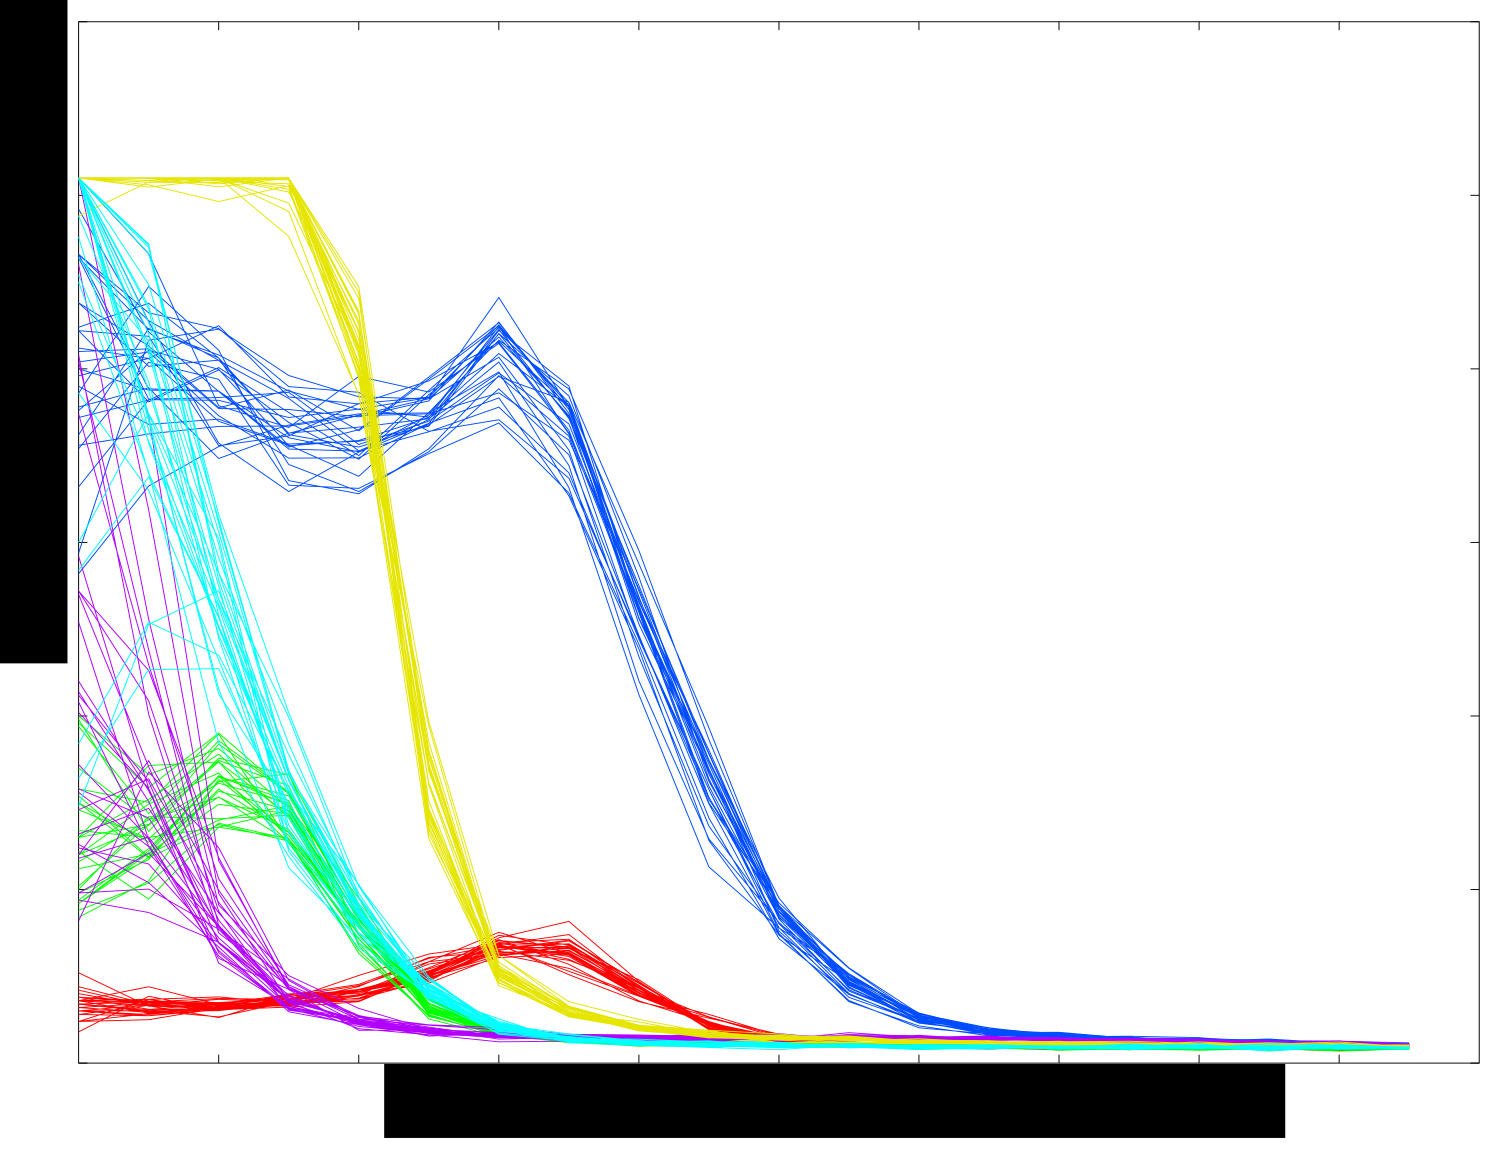
\includegraphics[width=0.99\linewidth]{images/AllLaserPersonalities_OneSpot.png}

\vspace{-0.1in}
\caption{\label{figure:six_laser_personalities} This figure shows 30
  personality measurements for each of 6 lasers from a single
  calibration screen location. A single data point (a laser
  personality measurement) is represented by a radial histogram of
  intensities arranged by distance from the centroid of the laser
  spot, and each line represents one such data point. Each laser is
  represented by a different color. The intensity measurements range
  from 0 to 255 (y-axis), and the distances from the centroid of the
  laser spot range from 0 to 20 (x-axis). As an example, the blue
  laser's spot reaches its peak intense approximately 6 pixels from
  its center.
}
\end{figure}


\subsection{Identifying Laser Spots: Matching Personalities}

Once calibration is complete, the system is able to match any laser
spot on the projection surface with one of the calibrated lasers.
When a laser spot is detected, its personality is calculated, and
matched with that of one of the known lasers.

For efficiency, we utilize two passes to process the camera image.  In
a first coarse pass, we examine every $n$th pixel in the camera image
and all pixels greater than a pre-set intensity threshold continue to
the second pass.  In the second pass, a generous window around each
seed pixel is examined.  We collect all nearby pixels above the
threshold and extract the largest connected component.  The centroid
of this component is set as the laser spot position.  We then compute
the histogram of pixel intensities shown in
Figure~\ref{figure:six_laser_personalities}.  The final task is to
match the detected histogram to the library of known lasers.  We do
this matching by calculating the sum of squared differences between
the detected histogram and the histogram of each each known laser.  We
then assign the laser ID as the minimum of these sums.  


% The raw intensity calibration data and best fit ellipse for each laser
% is shown in Figure~\ref{figure:laser_data} a) and Equation~\ref{equation:InitialNormalization}.  
% \begin{equation}
%   b_{norm} = \displaystyle\frac{b}{\displaystyle\sum_{L} \displaystyle\sum_{G} \displaystyle\sum_{I} }
%   \label{equation:InitialNormalization}
% \end{equation}
% where $b_{norm}$ is the normalized brightness value, $b$ is the brightness data point, and $L$, $G$, and $I$ are the 
% sets of all lasers, grid points, and samples. The process is similar for radius values.
% The scatterplot nature
% of this visualization may not look promising at first for robust
% identification of the laser signatures; 

It is important to note that the apparent laser intensity varies
spatially for each laser due to a number of additional variables,
including: distance from laser to screen, distance from screen to
camera, and camera vignetting.  We can easily normalize for these
variations.  First, we normalize for the camera position by averaging
all of the intensity data for all of the lasers collected at each of
the calibration grid points, and normalize the input by dividing it by
the spatial average.  We use barycentric coordinates and interpolation
to normalize laser points between calibration grid locations.  Camera
position normalization is especially crucial when the camera is placed
at an extreme angle to the screen, and thus experiences significant
perspective distortion.

%This normalization is shown in
%Figure~\ref{figure:laser_data} b) and is described in
%Equation~\ref{equation:InitialNormali

%zation}.  
% \begin{equation}
%   b_{norm_{SPATIAL}} = \displaystyle\frac{b}{\displaystyle\sum_{L} \displaystyle\sum_{I} }
%   \label{equation:SecondNormalization}
% \end{equation}
% The spatial
% normalization will remove the bulk of the cause of variation for the
% detected points from each laser, {\em assuming all lasers originate
%   from the same point within the room}.  
% 

Just as the camera position relative to the screen is important, the
laser spots also exhibit perspective distortion when they are used at
extreme angle to the screen.  We can similarly normalize for this
distortion, assuming that the intensity calibration data for each
laser is collected from a position near that laser's use location.

\subsection{Temporal Coherence and Simultaneous Use}

For the tests presented in this paper and companion video we do not
leverage temporal coherence in our detection.  Because the camera
image and laser output contain some noise, the quality of the
personality measurements and identification would benefit from
averaging the output of multiple frames known to be the same laser
from the tracking algorithm in Section~\ref{section:systemdetails}.

When multiple lasers are simultaneously detected on the screen, we can
leverage this information to disambiguate lasers with somewhat similar
histogram personalities.  We employ the Kuhn-Munkres algorithm to
assign unique labels to all detected points; that is, no two lasers
will be assigned the same ID, even if they both select the same ID as
their first choice.

%\fbox{2nd use of kuhn munkres}

%\fbox{classroom vs other use}




\section{Accuracy Testing}
\label{section:TestResults}
% SAY IN HERE THAT 92% FALL IN THE HIGHEST PERCENTAGE, AND 100% FALL IN THE HIGHEST TWO PERCENTAGES, WHEN TALKING ABOUT LASER ACCURACY AMONG THE 6 LASERS...GET THE PERCENTAGES FROM BARB'S CODE

We performed several tests to judge various notions of accuracy of the
\emph{laser personality} system. The tests were performed using six
lasers (given IDs 1-6) in the 19' x 23' space shown in Figure
\ref{figure:laser_testing_room_diagram}. The space was divided into a
series of testing locations, marked with an 'X' in the diagram, at
discretized $22.5\,^{\circ}$ arcs with radii of 5', 10', and 15' from
the center of the projection surface.

Two sets of calibration data were collected. For the first calibration
(referred to from now on as calibration $C1$), all six lasers were
calibrated from the 15' mark along the line perpendicular to the
projection surface (point A in Figure
\ref{figure:laser_testing_room_diagram}). For the second set of data
(calibration $C2$), all six lasers were calibrated simultaneously from
different points along the 10' arc (point B resides on this arc). The
accuracy of a laser was defined as the percentage of frames in which
the laser was identified correctly out of all detection frames. These
results are presented in Table \ref{table:AccuracyTestingResults}.

%PLACEHOLDERS!
\begin{figure}
  \centering
  \includegraphics[width=0.99\linewidth]{images/room_diagram_annotated.png}
  \caption{\label{figure:laser_testing_room_diagram} A diagram of the testing space. 'X's are marked in arcs at intervals of 5' 
from the center of the projection surface, separated by $22.5\,^{\circ}$ arcs. Five locations (A through E) are marked on the diagram for reference. }
\end{figure}


\begin{table*} [t]
\centering

\begin{tabular}{ | c | r | r | r | r | r | r | r | r | r | r | }
 \hline
 \textbf{Laser} & \multicolumn{2}{|c|}{\textbf{Single Position}} & \multicolumn{2}{|c|}{\textbf{Arc Movement}} & \multicolumn{2}{|c|}{\textbf{Line Movement}} & 
                  \multicolumn{2}{|c|}{\textbf{Walking Path}} & \multicolumn{2}{|c|}{\textbf{All Lasers}} \\
 \hline
  1 & 100.00\% & 100.00\%& 96.54\% & 98.27\% & 53.88\% & 74.14\% & 51.13\% & 68.49\% & 99.79\% & 100.00\% \\
  2 & 100.00\% & 100.00\% & 100.00\% & 100.00\% & 90.43\% & 95.21\% & 78.65\% & 86.25\% & 99.07\% & 100.00\% \\
  3 & 95.85\% & 100.00\% & 70.96\% & 73.48\% & 35.14\% & 48.65\% & 60.50\% & 96.10\% & 83.49\% & 98.75\% \\
  4 & 92.79\% & 100.00\% & 77.40\% & 100.00\% & 80.41\% & 100.00\% & 83.02\% & 100.00\% & 99.61\% & 99.78\% \\
  5 & 99.67\% & 99.67\% & 100.00\% & 100.00\% & 57.99\% & 92.57\% & 82.95\% & 94.26\% & 99.80\% & 99.92\% \\
  6 & 90.33\% & 96.03\% & 93.89\% & 95.91\% & 72.56\% & 79.70\% & 91.81\% & 94.86\% & 84.08\% & 99.90\% \\
  \hline
  \textbf{Min. Frames} & 521 & & 347 & & 230 & & 645 & & 968 & \\
 \hline  
\end{tabular}


\caption{\label{table:AccuracyTestingResults}Results from accuracy
  tests. Five tests were performed in all, and for each test and for
  each laser two percentages are reported: the percentage of frames in
  which it was correctly identified as its primary ID (left column), and the
  percentage of frames in which it was identified as either the primary or secondary
  ID (right column). The minimum number of frames collected for each test is reported
  along the bottom row. }

\end{table*}

%During testing, a concerted effort was made to maintain a consistent
%number of data collection frames within each test, and so 
The minimum number of frames considered for each test is reported in
Table~\ref{table:AccuracyTestingResults} along the bottom row. Five
accuracy tests were run in total, with users stationary, walking in an
arc, walking along a straight line, walking along a path, and using
all lasers simultaneously. For the tests, we count the number of times
the laser is correctly identified as the primary choice, and the number of times the correct
laser is the secondary choice (the laser intensity histogram with the
next smallest sum of squared differences). These two values comprise
the two columns in Table \ref{table:AccuracyTestingResults} for each
test, with the primary ID on the left and the secondary on the right.

\subsection{Description of Tests}

The first four tests all used calibration data $C1$, while the final
test used calibration data $C2$.

\textbf{Stationary Test} The purpose of this test was to judge how
well lasers could be matched to the calibrated data. Data was recorded
from the position at which the calibration $C1$ was collected,
position A, and the tester did not move from that location. Each laser
was shone on the screen for at least 521 frames (roughly 17.75
seconds), making sure to point at both the middle and each of the four
corners of the screen. Each laser was correctly identified in at least
90\% of the frames taken, and each laser was either identified
correctly or as the secondary laser at least 96\% of the time.

\textbf{Arc Walking Test} The purpose of this test was to judge how
much side-to-side movement affected the overall accuracy of the
identification system, because the shape of the laser spot is skewed
when seen from an angle, changing the laser's personality. Data was
recorded while users walked along the 10' arc of data collection
points, passing right-to-left through point B. The laser was kept as
close to the center of the screen as possible to avoid affecting the
laser spot in additional ways. Each of these tests lasted at least 347
frames (roughly 11.5 seconds). Four of the lasers performed well (with
at least 93\% accuracy), while lasers 3 and 4 maintained 70\%
accuracy. Each laser was identified as either its first or second
choice laser ID in at least 93\% of the frames, except laser 3.

\textbf{Straight Line Walking Test} The purpose of this test was to
judge how much distance from the screen affected the overall accuracy
of the system. Changing the distance to the projection surface changes
the radius and intensity of the laser spot, and thus affects the
histogram of the laser's personality. For this test, the user stood as
far from the screen as possible (approximately 20') and walked forward
to the 5' mark, perpendicular to the screen. The laser was once again
kept as close as possible to the center of the screen. Each of these
tests lasted at least 230 frames (roughly 7 seconds). The results for
this test were significantly poorer than other tests, as three of them
scored below 60\% (laser 3 scored below 40\%).
% This was the only test
%in which one of the lasers was more often identified as its secondary
%ID (laser 3) than its primary.

\textbf{Path Walking Test} The purpose of this test was to provide an
overall averaging of the previous two tests, and to mimic movement
expected by users in real-world environments. The path taken followed
the letters marking room positions in Figure
\ref{figure:laser_testing_room_diagram} from position A to B, C, D, E,
and back to A. The laser was again kept as close as possible to the
center of the screen. Each of the tests lasted at least 645 frames
(roughly 19.5 seconds). In general, the lasers performed as expected,
an average somewhere between the arc and the straight line tests. Only
laser 1 fell below 60\% accuracy, while none of the other lasers beside laser 1 had more
than 15\% failure to be the first or second choice histogram
personality.

\textbf{All Lasers Simultaneous Test} The purpose of the final test
was the assess how accurately the laser identification system
performed when several lasers were on the screen at once. In this
test, users stood at each of 6 marks along the 10' arc (the positions
from which calibration $C2$ data was collected) and all shone lasers
at the screen simultaneously. The laser spots followed a path that
touched all four corners as well as the middle of the projection
surface.  Two lasers, 3 and 6, were confused with one another in
approximately 15\% of the frames, but each of the other 4 lasers were
at least 99\% accurate.

\subsection{Results and Discussion}

Overall, our laser identification system is effective and useful for a
variety of applications. It is overwhelmingly effective when lasers
remain in the general area from which their calibration data is
collected while the system is in use. It is rare that a laser is
mislabeled in this instance. Many multi-user applications do not
require users move around the room while the system is in use, such as
education applications in a classroom environment, or games played
collectively by an audience. However, when moving from place to place,
the shape of the laser spot can change dramatically, and so the
personality can as well. As is to be expected, this is most extreme
when moving a different distance from the projection surface, as the
spot's intensity signature changes and its radius grows and shrinks
dramatically, making histogram comparison considerably more difficult.

These tests bring to light two significant shortcomings of our
identification system. The first is that position is important when
comparing a laser spot to a given set of laser personalities,
especially distance from the projection surface. The farther one moves
from the spot of calibration, the less accurate the laser
identification becomes. However, even in tests where the distance to
the screen changed, most of the lasers performed well. The system's
second shortcoming is that a laser's personality changes over the time
of its use. Battery-powered laser pointers change the range of their
output intensities as their batteries drain and the lasers themselves
warm up. Therefore, it is often the case that, over the course of its
use, a laser's personality will shift away from the data collected
during the calibration phase. Both of these shortcomings can be
addressed by the idea of continuous calibration, discussed in Section
\ref{section:FutureWork}.
%
%In addition, the addition of smart temporal coherence to the system would improve the 
%the fact that many of the tests in which lasers scored low as the primary saw a vast improvement when the laser was allowed to be 
%identified as the secondary laser points to the idea that many of the issues can be resolved with 

\section{Applications}
\label{section:Applications}

We have implemented a series of five applications that effectively
take advantage of multi-user interfaces for visualization, education,
and problem-solving. The common thread among each of the applications
is its use of input from several different users to achieve a common
goal, e.g. exploration of a data visualization or solving a
puzzle. Our applications are a multi-user painting program, a puzzle
solving program, a terrain and hydrography data visualization tool, a
graph visualization tool, and an infrastructure map visualization
tool. In each application, laser points are identified using their
\textit{personalities}, as described in section
\ref{section:LaserPersonalities}.

\subsection{Goal-Oriented Group-Based Problem Solving}

\begin{figure}[t]
  \begin{center}
  \begin{minipage}{0.99\linewidth}
    \includegraphics[width=0.99\linewidth]{images/paint.jpg}   
  \end{minipage}
  \end{center}
  \caption{\label{figure:paint}A visualization of the multi-user paint program demonstrating two-user collaboration. 
Notice that laser \#1 has currently been assigned the color white and is filling in the cloud, while laser \#2 has 
recently selected the ``undo'' function which removed its color assignment.}
\end{figure}

An aim of our multi-user interface is creating an environment that
simplifies goal-oriented group-based problem solving. To demonstrate
this idea, we present two applications that use the group dynamic to
collectively reach a goal. The first is our paint program, which
allows any number of users to paint on the screen using the laser
pointer as a brush, seen in Figure \ref{figure:paint}. Colors are
selected from a tablet of choices on the right side of the screen, and
each user can select his own. The ID of the laser that has selected a
color is displayed in the color button, telling the user which color
he has currently selected. Each pointer is identified when it is
detected on the painting surface portion of the screen, and the stroke
gesture made by the pointer creates a curve along the trajectory of
the gesture in the laser pointer's chosen color. There are also
buttons on the interface to increase and decrease line width, clear
the painting surface, and undo the last action performed by a
particular laser. Identifiable lasers are important for the paint
application, as it allows each user to manipulate the same canvas
while each drawing in his own color, making collaborative images easy
to create.

\begin{figure}[t]
  \begin{center}
  \begin{minipage}{0.99\linewidth}
     %a)
    \includegraphics[width=0.49\linewidth]{images/puzzle1.jpg}
     %b) 
    \includegraphics[width=0.49\linewidth]{images/puzzle2.jpg}
  \end{minipage}  \\
  \begin{minipage}{0.99\linewidth}
    % c) 
    \includegraphics[width=0.99\linewidth]{images/puzzle3.jpg}     
  \end{minipage}  \\
  \begin{minipage}{0.99\linewidth}
    %d) 
    \includegraphics[width=0.49\linewidth]{images/puzzle4.jpg}
    %e) 
    \includegraphics[width=0.49\linewidth]{images/puzzle5.jpg}
  \end{minipage}  
  \end{center}
  \caption{\label{figure:puzzle} A visualization of the puzzle application, in which five users (each represented 
by his own color) attempt to solve a 7x5 piece puzzle. The five images represent five points in time during the solving 
of the puzzle. Each border between two tiles that should not be adjacent is greyed out (top left image), but once a 
tile is placed next to its proper neighbor, the border fills in (middle image). Notice how the group has worked to 
assemble various pieces of the puzzle individually before finally moving them to the correct areas of the board.}
\end{figure}

To demonstrate a goal-oriented user interface, we present a puzzle
solving program, which reads in an image and breaks it up in to $n$
equally-sized rectangular textured tiles, randomizes them, and
displays the new order on the screen, seen in Figure
\ref{figure:puzzle}. The common goal of the users of this application
is the reassemble the original image by clicking and dragging the
tiles. Each tile consists of a central space (the majority of the
tile) which displays that tile's portion of the image, and a faded
border. The user must hover the laser pointer over a tile for
approximately a second before it is selected, which is indicated by
the faded border being filled in with the user's laser's assigned
color (each laser pointer is assigned its own unique color as it
enters the system). When two tiles the system knows to be adjacent are
placed in the proper order, the adjacent borders fill in, completing
that portion of the image. 

In our informal play with this application we found that users highly
enjoyed the game and used verbal communication in addition to the
joint editing to more quickly solve the puzzle.  Users commented that
each program's use of the laser pointer as an interaction device is
intuitive, and users in general became comfortable with the interface
with very little instruction.  However, we did observe some {\em
  trouble-makers} who sneakily and intentionally disassembled the
puzzle.  Since the application can identify laser pointers, it can
track the productivity and positive contribution of each user.
%is aware of how constructive or not each user is with
%regard to solving the puzzle, and so can provide feedback as part of
If specific users repeatedly make destructive actions, this user's
privilege in the system can be decreased and their actions ignored.
%the collaborative process where it scores each user on how helpful he
%was in finding the correct solution, or by punishing users who are
%continually destructive.
%


\subsection{Hydrography Visualization}


\begin{figure}[t]
  \begin{center}
  \begin{minipage}{0.99\linewidth}
     %a)
    \includegraphics[width=0.49\linewidth]{images/terrain1.jpg}
     %b) 
    \includegraphics[width=0.49\linewidth]{images/terrain2.jpg}
  \end{minipage}  \\
  \begin{minipage}{0.99\linewidth}
    % c) 
    \includegraphics[width=0.99\linewidth]{images/terrain3.jpg}     
  \end{minipage}  \\
  \begin{minipage}{0.99\linewidth}
    %d) 
    \includegraphics[width=0.49\linewidth]{images/terrain4.jpg}
    %e) 
    \includegraphics[width=0.49\linewidth]{images/terrain5.jpg}
  \end{minipage}  
  \end{center}
  \caption{\label{figure:hydrographyVisualization} A visualization of our terrain hydrography exploration tool, 
which takes in as input a height field and visualizes it. Notice the channel highlighted by the top left image, 
and water flow down the channel in the top right and middle images. While user \#1 adds rain to the terrain, user 
\#3 begins to raise the land, damming the channel (lower left image), until the hydrography information has been 
updated and the water must flow around the newly formed dam (bottom right image). }
\end{figure}


Data manipulation in a multi-user environment can be a powerful teaching tool. To this end, we have implemented 
a visualization tool for terrain hydrography analysis, seen in Figure \ref{figure:hydrographyVisualization}.
The goal of the application is to allow for the exploration of terrain hydrography data by multiple users through 
a laser pointer interface. The application consists of a data view and a graphical user interface side-by-side, 
in which modes are selected in the GUI through dwell-selection. In addition to selection of modes, the laser 
pointers are also used to interact directly with the 3D terrain data and camera view.
%, depending on the current mode of the program.

The application takes as input a height field (a scalar field of height values arranged on a regular grid), 
which represents the terrain to be visualized. The terrain is drawn in the data view section of the display, 
color coded according to scalar value (height, in this case) and normalized to fit the range of maximum to minimum 
values of the data. The user selects a mode using buttons on the right side of the screen. These modes include 
camera position modes (Rotate, Translate, Zoom), visualization modes (Watershed and Channel Network), and 
interaction modes (Add Rain, Lower Land, Raise Land). Because each user can have any mode active at any given point in 
time, multiple updates to the data and visualization can occur simultaneously. When a button is selected, the application 
identifies the laser pointer that made the selection and associates it with the corresponding mode. For example, if laser 
\#3 selects the Rotate mode, a small ``3'' appears on the Rotate button and laser \#3 can now rotate the camera through a 
click-and-drag motion in the data view window.

Upon read in of the data (and every time it is altered by one of the
interaction modes), the hydrography information of the terrain is
determined using both a variation of the least-cost flow routing
method by Metz, et al.~\cite{hess-15-667-2011}, and the flow
accumulation method presented by O'Callaghan and Mark~\cite{O'Callaghan1984323}. The least-cost flow routing is fast
enough in its implementation to allow the hydrography information to
be updated in interactive time (approximately 15 to 20 FPS). This is
important, as interaction with the data and the camera view should not
impede exploration of the data by other users.

The camera position modes allow users to rotate, translate, and zoom the camera, changing the view of the data, as 
described above. Watershed and Channel Network modes both visualize hydrography information on the terrain surface. 
While in watershed mode, a laser point detected on the surface of the data highlights the watershed of the corresponding 
space on the data. When Channel Network mode is active, the channels of the terrain are visualized. 
%These two modes can be seen in figure \ref{figure:WatershedAndChannelNetwork}.
Finally, interaction modes allow the users to manipulate the
data. Raise and Lower Terrain modes allow the user to raise and lower
the surface data by selecting a space on the data. The data is
manipulated according to a radial Gaussian filter, centered at the
space selected by the laser. This, in essence, grows hills and
craters. When Add Rain mode is selected, the user can select a space
on the terrain, and rain drops fall onto the surface in a radial
pattern centered at the selected space. The rain then flows, according
to the internal hydrography information, down hill and off the edge of
the terrain. These modes are demonstrated in
Figure~\ref{figure:hydrographyVisualization}.

The multi-user nature of the application allows some users to be manipulating the data itself, while others explore 
the repercussions of this manipulation (by creating rain drops and watching where they flow and highlighting various 
watersheds along the path of the flowing water), all while others manipulate the camera, perhaps following the path 
of the water as it flows between mountains and off the edge of the terrain. Users have commented informally that the 
ability to manipulate the surface data while watching rainwater flow across the terrain was particularly useful, as 
it demonstrated how much hydrography can change with slight alterations to the terrain.

\subsection{Spatial Network Visualization}

\begin{figure}[t]
  \begin{center}
  \begin{minipage}{0.99\linewidth}
     %a)
    \includegraphics[width=0.49\linewidth]{images/graph1.jpg}
     %b) 
    \includegraphics[width=0.49\linewidth]{images/graph2.jpg}
  \end{minipage}  \\
  \begin{minipage}{0.99\linewidth}
    % c) 
    \includegraphics[width=0.99\linewidth]{images/graph3.jpg}     
  \end{minipage}  \\
  \begin{minipage}{0.99\linewidth}
    %d) 
    \includegraphics[width=0.49\linewidth]{images/graph4.jpg}
    %e) 
    \includegraphics[width=0.49\linewidth]{images/graph5.jpg}
  \end{minipage}  
  \end{center}
  \caption{\label{figure:graphVisualization} A visualization of our graph exploration application, in which a 
database with connectivity information is read in, displayed, and explored by users. In this instance, the data 
used is a taxonomic tree of animals. In the top row, the node ``Mammals'' is circled and expanded, visualizing 
the nodes from the next level down the sub-tree. The third level of this sub-tree is visualized in the center 
image (with pictures of each of the animals found in the database). In the bottom left image, you can see one 
user dragging a node while another user collapses one level of the tree, with the result of this operation seen 
in the bottom right image.}
\end{figure}

In addition to data visualization and manipulation, data exploration in a group setting is an important application 
of our multi-user laser interface. To demonstrate this, we present a graph visualization tool that allows users 
to explore data organized by nodes and edges, seen in Figure \ref{figure:graphVisualization}. Our application 
takes as input node and connectivity information. Laser points which dwell on a node for a period of time ``grab'' 
the node, indicated by the laser trail turning green, and can drag the node to a new location. The graph will 
rearrange itself based on a mass-spring simulation, minimizing the energy in the system. If there is a notion of 
``expansion'' that can be applied to the graph (such as with a tree) then the interface supports expansion and 
collapse operations. Our example dataset is a taxonomic database of animals, organized in a tree structure, so 
expansion in inherent in the data. To expand a node (such as the ``Mammals'' node, in our example), a circle 
motion is made around the node, and the next level of the subtree is exposed. To collapse a node (which reverses 
the expand operation), a squiggle or cross-out gesture is made. These operations can be seen in 
Figure~\ref{figure:graphVisualization}.


\begin{figure*}[t]
  \begin{center}
  \begin{minipage}{0.99\linewidth}
    \includegraphics[width=0.99\linewidth]{images/synenv_crop.jpg}   
  \end{minipage}
  \end{center}
  \caption{\label{figure:synenv} A visualization of our infrastructure data exploration and editing tool that 
demonstrates two users working interacting with the map's data. The GUI on the left allows users to select 
which nodes are visible, as well as select actions to take (bottom left corner) between point, select, pan, 
and draw. Selecting a node enlarges it to display the data found within, while panning moves the camera around 
the map. Draw allows the user to make annotations to the visualization, for the benefit of other users. }
\end{figure*}


Our final application is a visualization, exploration, and editing tool for
infrastructure data shown in Figure~\ref{figure:synenv}.
The data are organized as a spatial graph of interconnected nodes and arcs in several different infrastructure 
systems: electric power, telecommunications, transportation, etc. The tool is used to visualize the complex 
network along with vulnerabilities during hurricane and flooding scenarios (e.g., where are ambulances re-routed 
if a local hospital is flooded). 

Representatives from the different infrastructure systems
% (e.g.,power, water, sewer, communications, emergency personnel, etc.) 
can meet in the Emergency Response Organization control room and discuss
interdependencies between the networks.  It is important that the
interface be flexible, highly interactive, and intuitive 
%intuitive and have 
with a very minimal learning curve, since
in-depth training of these interfaces will not be practical in
disaster response situations.  The large format projection system with
laser pen interface is particularly applicable to this situation.
Tracking the identities of the users and their input to the system is
also critical.

% MORE DESCRIPTION HERE OF THE INTERFACE

Users may select and edit nodes and edges of the data, and each individual user's edits are saved, not only for 
logging purposes, but to save the state of each user, as similar to the hydrography visualization tool. 
This application demonstrates the potential advantages of a multi-user system in a real-world, fast-paced, 
problem-solving environment.

\section{Conclusion}

% REWORK TALKING ABOUT HISTOGRAM
Multi-user interaction on large-scale displays is a powerful
collaborative tool with several applications. In this paper, we have
presented a method for identifying off-the-shelf laser
pointers in an inexpensive and simple manner by calibrating each laser
pointer's IR spillover's intensity histogram, called the laser's
\emph{personality}, allowing for closest-neighbor matching of data
points. The system requires only a calibration step to set up, and
once it is complete multiple users can interact with interfaces in a
large-scale environment. Applications tailored to multi-user
collaborate problem solving efforts are presented in this paper that
take advantage of our system's ability to identify laser points to
explore data, manipulate data, and solve problems in a group
environment. Our method is inexpensive, accurate, simple, and scalable
to large screen displays.

\subsection{Limitations and Future Work}
\label{section:FutureWork}

% REWORK TALKING ABOUT HISTOGRAM, MAKING RADIAN BINS, ETC. ALSO, CONTINUOUS CALIBRATION
%In the future, our system will be improved by fitting a more complicated model to the radius and brightness data. 
%More complicated shapes, such as asymmetric shapes, would be more accurate as not all lasers behave symmetrically with 
%regard to their brightness and IR radius, and so an elliptical Gaussian is rarely the best fit. Along the same lines, 
While the system works well when users do not change how far they are from the project surface (sufficient for 
many applications), there are times when this is not enough. One clear extension to this work is the introduction 
of continuous calibration. First, we will omit the special calibration step, and instead generate initial 
calibration from early incidental usage, and continue to dynamically update a laser's data as it is used. As 
new data is added to the system, older data will be replaced, and so the calibration data will change as the 
lasers' personalities do. This continuous update of the calibration data will allow for less confusion between 
laser spots as the laser points warm up and change from continuous usage. 
%In addition, calibration of the spot radius will be made faster so as to allow for the dynamic updates, which 
%will allow for the environments in which the system is used to be extended to more useful spaces, such as a 
%classroom. We will also collect and analyze accuracy data, allowing us to measure improvement in the system as we make the noted additions.

Our applications will also be improved. One such improvement would be a move to a multiple-screen multiple-camera 
format. Laser strokes will need to be ``passed off'' accurately from one camera's view to the other's, and each 
viewing system will need to be calibrated independently (unless dynamic calibration is implemented). We will also 
extend our applications to more fully take advantage of identifiable laser points. For instance, we will create 
a user feedback system for the puzzle application, in which users who are contributing will be rewarded while 
those who are destructive may face a penalty to their piece-moving privileges. This would mimic real-world collaborative reward systems.

%% if specified like this the section will be omitted in review mode
\acknowledgements{
Thank you to Andrew Dolce, for his contributions to the laser-recognition code. Thank you to Dr. W. Randolph Franklin, 
for his implementation of the least-cost flow routing hydrography method. Thank you to Patrick Phipps for his work on 
the map visualization application and his graph data structure code, and thank you to Andrew Zonenberg for his work on 
the map visualization application. Thank you to Joshua Nasman for his help with application testing, posing, and proof 
reading. Thank you to Ryan Baltazar for his ellipses-fitting code. Thank you to Ted Yapo for his work on camera calibration.}

\bibliographystyle{abbrv}
\bibliography{GI2012}
\end{document}
